\documentclass{beamer}

\usetheme{Madrid}      % 内置主题(推荐新手使用)
\useoutertheme{miniframes} % 外层主题:横向小方块目录条
% \usetheme{Frankfurt}
% \usepackage[x11names]{xcolor}  % 加载扩展色库
% \usecolortheme[named=OliveDrab3]{structure}  % 柔和绿色
\setbeamercolor{structure}{fg=teal!70!black} % 导航条主色(可改)
\usepackage{graphicx}
\usepackage{amsmath}
\usepackage{caption}

\title{Wavelet Transform for Image Processing}
\author{
\texorpdfstring{
Zhang Jinrui\thanks{alternative email:zhangjr1022@mails.jlu.edu.cn}
\\
Mo Zian
}
{
Zhang Jinrui\thanks{alternative email:zhangjr1022@mails.jlu.edu.cn}
,
Mo Zian
}
}
\date{\today}

\begin{document}

\frame{\titlepage}  % 首页封面

\section{Haar wavelet}
\begin{frame}
    For a \(2^{N}\) points sequence, the mother
    wavelet is
    \[
        \psi(n) =
        \begin{cases}
            0,                     & \text{if } n < 0               \\
            \frac{1}{\sqrt{2^N}},  & \text{if } 0\leq n < 2^{N-1}   \\
            \frac{-1}{\sqrt{2^N}}, & \text{if } 2^{N-1}\leq n<2^{N} \\
            0,                     & \text{if } n >= 2^N            \\
        \end{cases}
    \]
    We have
    \[
        \langle\psi,\psi\rangle=\sum_{k=0}^{2^N-1}\frac{1}{2^N}=1
    \]
\end{frame}
\begin{frame}
    For other derived basis we use
    this discretized formula
    \[
        \psi_{j,k}(n)=\sqrt{2^j}\psi(2^j(n-2^{N-j}k)) , 0\leq j\leq N-1
        , k<=2^j-1
    \]
    \[
        \left[
            \begin{array}{cccc}
                \psi_{0,0}   & 0            & \cdots     & 0                    \\
                \psi_{1,0}   & \psi_{1,1}   & \cdots     & 0                    \\
                \psi_{2,0}   & \cdots       & \psi_{2,3} & 0                    \\
                \vdots       & \vdots       & \ddots     & 0                    \\
                \psi_{N-1,0} & \psi_{N-1,1} & \cdots     & \psi_{N-1,2^{N-1}-1}
            \end{array}
            \right]
    \]
    And a average basis as following
    \[
        \phi(n) =
        \begin{cases}
            0,                    & \text{if } n < 0               \\
            \frac{1}{\sqrt{2^N}}, & \text{if } 0\leq n < 2^{N-1}   \\
            \frac{1}{\sqrt{2^N}}, & \text{if } 2^{N-1}\leq n<2^{N} \\
            0,                    & \text{if } n >= 2^N            \\
        \end{cases}
    \]
\end{frame}
\begin{frame}
    there are
    \[
        1+\sum_{k=0}^{N-1}2^k=2^N
    \]
    basis.
    which will be \(2^N\) coefficients
    then every \(2^N\) sequence \(f(n)\) can be written as
    \[
        f(n)=a\phi(n)+\sum_{j=0}^{N-1}\sum_{k=0}^{2^j-1}c_{j,k}\psi_{j,k}
    \]
    Then each coefficients can be obtain by inner product.
    \[
        a=\langle f(n),\phi(n)\rangle
    \]
    \[
        c_{j,k}=\langle f(n),\psi_{j,k}(n)\rangle
    \]
\end{frame}
\begin{frame}
    The inner product of two sequence are define as follow.
    \[
        \langle f(n),g(n)\rangle=\sum_{k=0}^{2^N-1}f(k)g(k)
    \]
    the transformed sequence \(\hat{f}(n)\)
    satisfies
    \[
        c_{j,k}=\hat{f}(2^j+k)
    \]
    \[
        a=\hat{f}(0)
    \]
\end{frame}

\section{Image compression}
\begin{frame}
    \frametitle{Image compression}
    Let's see an application with Haar wavelet first.\\ \ \\
    By our research, $\forall\ m \in \mathbb{N}_{+}$, we can get \textbf{an set of orthonormal bases} of $\mathbb{R}^{m}$ quickly.
    \begin{block}{Theorem 2.1}
        Let $\{u_{i}\}_{i=1}^{m}$ is a set of \textbf{orthonormal bases} of $\mathbb{R}^{m}$, $\{v_{i}\}_{i=1}^{n}$ is a set of \textbf{orthonormal bases} of $\mathbb{R}^{n}$, then
        $$\{u_{i}\times v_{j}\ |\ i = 1,\cdots m, j=1,\cdots n\}$$
        is a set of \textbf{orthonormal bases} of $\mathbb{R}^{m\times n}$.
    \end{block}
\end{frame}
\begin{frame}
    \frametitle{Image compression}
    A grayscale image is stored as a grayscale matrix in the computer. Then we only need to know how to "{\color{blue}compress}" a matrix.\\ \ \\
    For $A \in \mathbb{R}^{m\times n}$, if $\{u_{i}\},\{v_{j}\}$ are sets of \textbf{orthonormal bases} of $\mathbb{R}^{m}$ and $\mathbb{R}^{n}$, according to (\textit{Theorem 2.1}),
    $\exists\ \omega_{i,j}\in\mathbb{R}, i = 1, \cdots m, j = 1, \cdots, n,$
    $$	A = \sum_{i,j}\omega_{i,j}\ \cdot \ u_{i} \cdot v_{j}^{T}.$$
    Let $M = (u_{1},u_{2},\cdots,u_{m}),\ N = (v_{1},v_{2},\cdots,v_{n}), W = (\omega_{i,j}).$ Then
    $$M^{T}AN =W,\ MWN^{T} = A.$$
\end{frame}
\begin{frame}
    \frametitle{Image compression}
    {\color{red}If $\omega_{i,j}$ is too small, the influence of  corresponding basis can be ignored.} \\Then
    \begin{align*}
        \widetilde{A} = \sum_{i,j}\widetilde{\omega_{i,j}}\ \cdot \ u_{i} \cdot v_{j}^{T},\ \widetilde{\omega_{i,j}} = \left\{
        \begin{aligned}
             & \omega_{i,j}, & \ |\omega_{i,j}| > \lambda    \\
             & 0,            & \ |\omega_{i,j}| \leq \lambda
        \end{aligned}
        \right..
    \end{align*}
    $\widetilde{A}$ is an approximation of $A$, while $\lambda$ is image compression strength.\\ \ \\
    Let $\widetilde{W} = (\widetilde{\omega_{i,j}}).$ As long as $\lambda$ is large enough, we can transform $\widetilde{W}$ into a \textbf{sparse matrix} which needs less storage space.\\ \ \\
    {\color{blue}Then we set $\lambda$ equal to $0.5$ and see the result.}
\end{frame}
\begin{frame}
    \frametitle{Image compression}
    \begin{figure}[ht!]
        \centering
        \begin{minipage}{0.45\textwidth}
            \centering
            
\includegraphics[width=0.9\textwidth]{fig/Siakam_gray.png} % first figure itself
            \caption{Original image}
            % \label{fig:Haar_sin}
        \end{minipage}\hfill
        \begin{minipage}{0.45\textwidth}
            \centering
            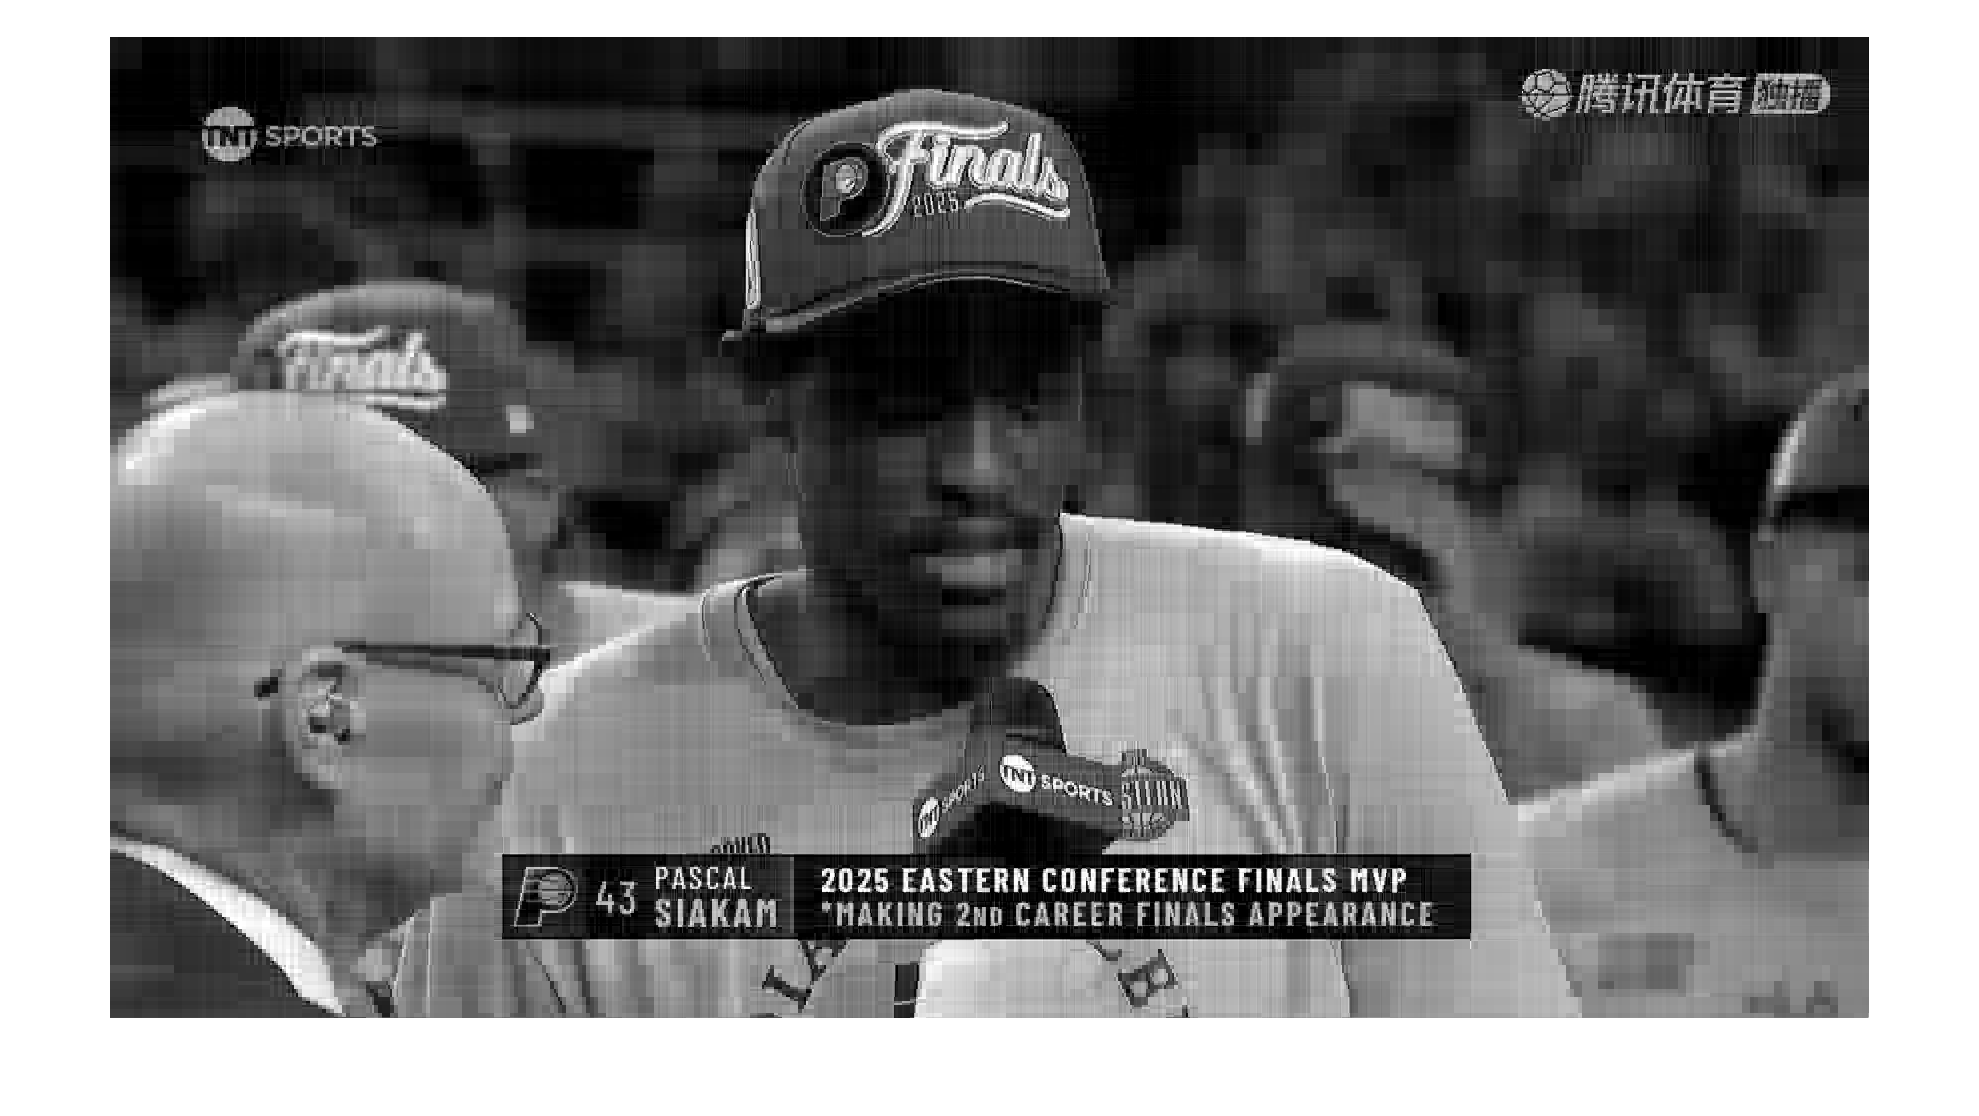
\includegraphics[width=0.9\textwidth]{fig/Siakam_compressed.png} % second figure itself
            \caption{Final image}
        \end{minipage}
    \end{figure}
\end{frame}
\begin{frame}
    \frametitle{Image compression}
    For original image , the size of stored information is $981\times1759 = 1725579$. \\\ \\
    {\color{red} However, after compression, the size of stored information is  only $15364\times2 = 30728$.} \\\ \\
    Indeed, we reduce storage space by compression. However, we also lose much detailed information of original picture. That's why we should change $\lambda$ for different purposes to reach the balance.
\end{frame}




\end{document}
